\documentclass[12pt,a4paper,parskip=full]{scrartcl}
\usepackage{float}
\usepackage[default,scale=1]{opensans} 

\usepackage[T1]{fontenc}

\usepackage[margin=2.4cm]{geometry}
 \geometry{a4paper}

\usepackage{xcolor}
 \definecolor{red}{HTML}{cc0000}
 \definecolor{gray}{HTML}{666666}

\usepackage{sectsty}
 \sectionfont{\color{red}}
 \subsectionfont{\fontsize{25}{25}\color{red}}
 \subsubsectionfont{\fontsize{20}{20}\color{red}}
 \renewcommand{\labelitemi}{$\cdot$}
 \renewcommand{\labelitemii}{$\cdot$}
 \makeatletter
 \let\latexl@section\l@section
 \def\l@section#1#2{\begingroup\let\numberline\@gobble\latexl@section{#1}{#2}\endgroup}
 \makeatother

\usepackage{graphicx}
 \graphicspath{{./../../images/}}

\usepackage{hyperref}

\usepackage[style=footnote-dw]{biblatex}
 \bibliography{S@SGuideBib}
 \setlength\bibitemsep{0.5\baselineskip}

\usepackage[hungarian]{babel}

\usepackage{enumitem}

\usepackage[T1]{fontenc}
\fontfamily{verdana}

%\usepackage{scrlayer-scrpage}{}
\usepackage{fancyhdr}
 \makeatletter
 \renewcommand{\@seccntformat}[1]{}
 \makeatother
 \setlength\parindent{0pt}{}
 \pagestyle{fancy}
 \fancyhf{}
 \lhead{ \fancyplain{}{A Scrum At Scale Útmutató}}
 \rfoot{ \fancyplain{}{\thepage} }
 \lfoot{\textcopyright 2006-2022 Jeff Sutherland \& Scrum Inc.}


% Definition of title page - (needs different documentclass)
\makeatletter
  \renewcommand{\maketitle}{\begin{titlepage}
    \begin{center}
      \makebox[\textwidth]{\fontsize{40}{40}\selectfont{\color{red}\@title\textsuperscript{\textbf{\textregistered}}}}\\
      \vspace{0.5cm}      	
      \fontsize{20}{20}\selectfont{\color{gray}\@subtitle}
    \end{center}
    \vspace*{1cm}
    \begin{figure}[H]
      \centering
      
\includegraphics[scale=1]{Cover.png}
    \end{figure}
    \begin{center}    
      \small {
        Verzió \version -- \@date \\
        \vspace{0.3 cm}
        Fordítás verziója \translationver
      }
    \end{center}
    \vspace{2.5 cm}
    \begin{center}
      \footnotesize{
        ©2006-2022 Jeff Sutherland and Scrum Inc., All Rights Reserved\\
        Scrum@Scale is a~registered trademark of Scrum Inc.\\
        Released under Creative Commons 4.0 Attribution-Sharealike License
      }
    \end{center}
  \end{titlepage}
}
\makeatother


\title{\Huge{\color{red}\textbf{A Scrum At Scale
\textsuperscript{\registered} 
Útmutató}}}
\subtitle{\color{gray}Hiteles útmutató a Scrum@Scale keretrendszerhez:\\ A működő skálázás}
\author{-}
\date{2022. február}
\newcommand{\version}{2.1}
\newcommand{\translationver}{2025.03.19.}

\begin{document}
%\maketitle
\tableofcontents

\subsection{Előszó a Scrum@Scale Útmutatóhoz}\label{preface-to-the-ScrumatScale-guide}

A Scrum, ahogyan azt eredetileg a Scrum Útmutató megfogalmazza, arra összpontosít, hogy egyetlen Scrum csapat képes legyen optimális értéket szállítani fenntartható tempóban. A létrejötte óta a Scrum használata kiterjedt olyan termékek, folyamatok és szolgáltatások létrehozására, amelyekhez több csapat erőfeszítésére van szükség.

Ismételten megfigyelték, hogy a való életben ahogy a Scrum csapatok száma nőtt egy szervezeten belül, két fő probléma merült fel:

\begin{itemize}%[label={\huge\textbullet}]
\itemsep10pt
\item
 A csapatok által szállított munkamennyiség, sebesség és minőség csökkenni kezdett olyan problémák miatt, mint a csapatok közötti függőségek, a munkák duplikálása és a kommunikációs többletköltségek.
\item
 Az eredeti menedzsment struktúra hatástalan volt az üzleti agilitás megvalósításában. Problémák adódtak, mint például versengő prioritások és a csapatok gyors átcsoportosításának képtelensége a dinamikusan változó piaci feltételekhez való alkalmazkodáshoz.
\end{itemize}

Ezeknek a problémáknak az orvoslására szükség volt egy olyan keretrendszerre, amely hatékonyan képes több Scrum csapat munkáját összehangolni, az alábbi célok elérése érdekében:

\begin{itemize}
\itemsep10pt
\item
 Lineáris skálázhatóság: A Scrum csapatok számának növekedésével arányosan növekvő munkatermék-szállítás.
\item
 Üzleti agilitás: A képesség arra, hogy gyorsan reagáljanak a változásokra, az eredeti stabil konfiguráció alkalmazkodásával.
\end{itemize}

A Scrum@Scale segít a szervezetnek arra összpontosítani, hogy több Scrum csapat hálózata együttesen prioritási célokat érjen el. Ezt úgy éri el, hogy egy olyan struktúrát alakít ki, amely természetes módon kiterjeszti az egyes Scrum csapatok működését egy hálózatban, és amelynek vezetői funkciója a minimálisan szükséges bürokrácián (MVB) alapul.

Egy hálózat akkor képes lineáris skálázhatóságot elérni, ha a jellemzői függetlenek annak méretétől. Egy ilyen csapathálózat megtervezése és koordinálása nem korlátozza a növekedést egy meghatározott módon; ehelyett lehetővé teszi a hálózat organikus növekedését, a szervezet egyedi igényei alapján, fenntartható változási tempóval, amelyet jobban elfogadnak az érintett egyének.

A minimálisan szükséges bürokrácia az a legkevesebb irányító testület és folyamat, amely szükséges egy szervezet funkcióinak ellátásához, anélkül hogy akadályozná az ügyfélérték leszállítását. Ez segíti az üzleti agilitás elérését a döntéshozatali késedelem (a döntéshozatalhoz szükséges idő) csökkentésével, amelyet a siker elsődleges mozgatórugójaként tartanak számon. A Scrum@Scale bevezetésének megkezdéséhez elengedhetetlen az Agilis Manifestó és a 2020-as Scrum Útmutató ismerete. Ha egy szervezet nem érti az agilitás természetét, nem lesz képes megvalósítani azt. Ha egy szervezet nem képes a Scrum-ot alkalmazni, akkor nem képes skálázni.

\subsection{A Scrum@Scale Útmutató célja}\label{purpose-of-the-ScrumatScale-guide}

Jelen Útmutató meghatározza a Scrum@Scale keretrendszer elemeit és azok definícióit. Megmagyarázza a skálázott szerepek felelősségi körét, eseményeket és (nagy)vállalati munkaanyagokat, valamint azokat a szabályokat, amelyek összefogják ezeket.

Az Útmutató négy alapvető részre tagolódik:

\begin{itemize}
\itemsep1pt\parskip0pt\parsep0pt
\item
 Bevezetés a Scrum@Scale-be, az elkezdéshez szükséges alapvetésekkel.
\item
 A Scrum Master Ciklus áttekintése.
\item
 A Product Owner Ciklus áttekintése.
\item
 A ciklusok összekapcsolásának áttekintése.
\end{itemize}

Minden egyes komponens meghatározott célt szolgál, amely elengedhetetlen a sikeres skálázáshoz. Alapvető szerkezetének vagy eszmeiségének megváltoztatása, elhagyása, vagy az ebben az útmutatóban lefektetett alapszabályok be nem tartása korlátozza a Scrum@Scale előnyeinek elérését.

Az alapszerkezeten és az egyes komponensek megvalósításának szabályain túlmutató konkrét taktikák eltérőek lehetnek, és azokat ez az útmutató nem ismerteti. Más források kiegészítő mintákat, folyamatokat és meglátásokat nyújtanak.

\subsection{Meghatározások}\label{definitions}

A Scrum egy olyan keretrendszer, amely kevés előírást alkalmazva segíti az embereket, csapatokat és szervezeteket, hogy komplex problémákra adaptív megoldásokkal értéket teremtsenek.

A Scrum Útmutató előírja azokat a minimális elemeket, amelyek megteremtik azt a csapatkörnyezetet, amely elősegíti az innovációt, az ügyfél elégedettséget, a teljesítményt és a boldogságot. A Scrum radikális átláthatóságot és formális események sorozatát használja arra, hogy a csapat lehetőséget kapjon működésük és termékeik megfigyelésére és az alkalmazkodásra.

A Scrum@Scale egy kevés előírást alkalmazó szervezeti keretrendszer, amelyben a Scrum Útmutatót következetesen alkalmazó csapatok hálózata képes komplex adaptív problémák megoldására, miközben kreatív módon a lehető legmagasabb értékű termékeket szállítják. Ezek a „termékek” lehetnek fizikai, digitális, komplex integrált rendszerek, folyamatok vagy szolgáltatások.

A Scrum@Scale Útmutató leírja a Scrum skálázásához szükséges minimális elemeket, és ebből fakadóan az egész szervezetre kiterjedő üzleti agilitást. Az útmutató alkalmazható minden típusú szervezetben: iparban, kormányzatban, nonprofit szervezeteknél vagy az akadémiai szférában. Ha egy szervezet még nem használja a Scrumot, a működési rendszerének módosítása szükséges.

A Scrum-ban különös figyelmet fordítanak a „mit” (termék) és a „hogyan” (folyamat) elszámoltathatóságának szétválasztására. Ugyanez a gondosság érvényesül a Scrum@Scale-ben is, hogy a felelősségi körök és az elszámoltathatóság egyértelműen meg legyenek határozva. Ez kiküszöböli azokat a szervezeti konfliktusokat, amelyek akadályozzák a csapatok optimális termelékenységét. 

Mivel a Scrum@Scale különálló komponensekből áll, lehetővé teszi a szervezet számára, hogy testre szabja a szervezet-, és működésfejlesztési stratégiáját és a transzformáció végrehajtását. Ezáltal egy szervezet célzottan priorizálhatja a változtatási erőfeszítéseket a legfontosabb vagy leginkább alkalmazkodásra szoruló területeken, és fokozatosan haladhat tovább a többi területen.

A Scrum@Scale ezeket a komponenseket két ciklusra osztja: a Scrum Master Ciklusra (a „hogyan”) és a Product Owner Ciklusra (a „mit”), amelyek két komponensnél metszik egymást, és egy harmadik komponensen osztoznak. Ezek a ciklusok összességükben egy erőteljes támogató struktúrát alkotnak több csapat közös erőfeszítéseinek összehangolásához egyetlen irányvonal mentén.

\subsection{A Scrum@Scale elemei}\label{the-components-of-scrumatscale}
\begin{figure}[H]
    \centering
    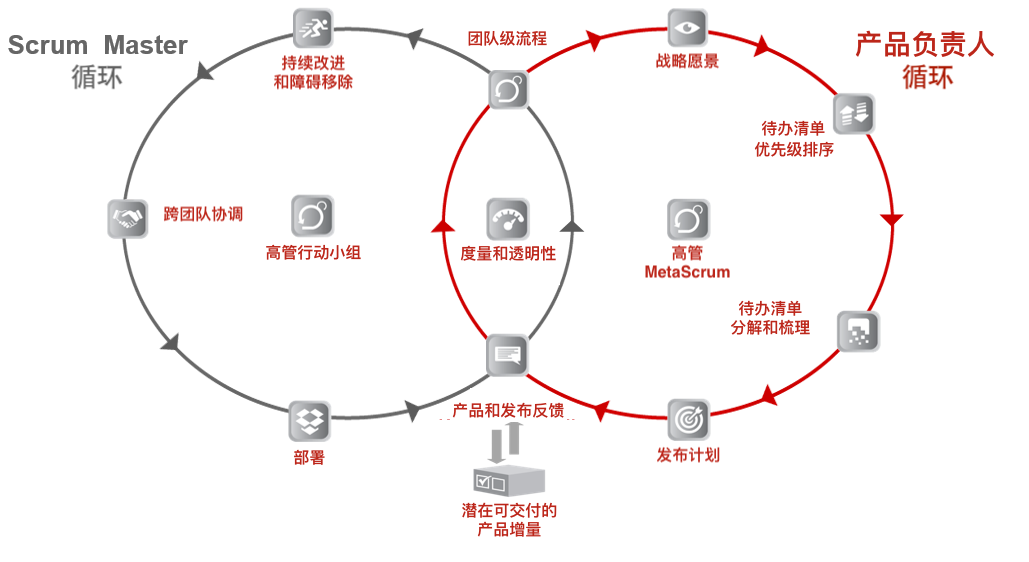
\includegraphics[scale=0.25]{SMPO-Cycle.png}
\end{figure}

\subsubsection{Értékvezérelt kultúra}\label{values-driven-culture}

A Scrum@Scale célja, hogy olyan egészséges szervezeti kultúrát építsen, mely az empirikus folyamatirányítás és a Scrum Értékek pillérein alapszik. Az empirikus folyamatirányítás pillérei az átláthatóság, megfigyelés és alkalmazkodás. A nyíltság, bátorság, fókusz, tisztelet és elkötelezettség, mint Scrum értékek, támogatják a pillérek megvalósulását.

A nyíltság támogatja az összes munka és folyamatok átláthatóságát, amely nélkül nem lehet azokat őszintén megfigyelni és megkísérelni a jobbá tételüket. A bátorság arra utal, hogy merész lépéseket kell tenni / ugrásokra van szükség ahhoz, hogy innovatív módokon, gyorsabban szállítsuk az értéket. A fókusz és az elkötelezettség utal arra, ahogyan kezeljük a munkából fakadó kötelezettségeinket, az ügyfél érték teremtést a legfontosabb prioritásként kezelve. Végezetül, mindennek egy olyan környezetben kell történnie, amely a munkát végző egyének tiszteletén alapul, akik nélkül semmi sem jöhet létre.

A Scrum@Scale úgy segíti a szervezeteket abban, hogy prosperáljanak, hogy pozitív, csapat szinten megjelenő tanulási környezetet teremt, ahol fenntartható tempóban dolgoznak, és ahol az ügyfélérték teremtés a legfontosabb.

\subsubsection{Kezdő lépések: Az Agilis Operációs Rendszer telepítése}\label{getting-started-installing-an-agile-operating-system}

Csapatok hálózatának implementálásakor kritikus fontosságú, hogy a skálázást megelőzően egy skálázható referencia-modellt dolgozzunk ki. A referenciamodell néhány olyan csapatból áll, amelyek minden Sprintben összehangoltan képesek eredményt előállítani. Ahogy ezek a csapatok sikeresen bevezetik a Scrumot, a szervezet többi része a Scrum egy működő, egészséges példáját tudja lemásolni. Ez prototípusként szolgál a Scrum skálázásához: az egymással közös értékteremtésben résztvevő csapatok hálózatának megalkotásához. A Scrum bevezetésének (csapat szintű) hiányosságai felnagyítódnak, ha több (egymással összefüggő) csapatban kerül bevezetésre a skálázott Scrum. Skálázási problémák lehetnek szervezeti irányelvek és folyamatok vagy fejlesztési gyakorlatok, amelyek blokkolják a teljesítményt és frusztrálják a csapatokat.

Skálázott környezetben a referencia-modell a legjobban úgy alkalmazható, ha olyan csapatokat csoportosítunk, amelyeknek össze kell hangolódniuk annak érdekében, hogy egy Scrum of Scrums (SoS) keretében teljesen integrált inkrementumokat tudjanak közösen szállítani. 

A hatékony működéshez a Scrum of Scrums-t csak a minimálisan szükséges bürokráciának (minimum viable bureaucracy, MVB) kell támogatnia, amely két vezetői csoportból áll: egy Executive MetaScrum (EMS) fórumból, amely arra összpontosít, hogy mit hoz létre a Scrum of Scrums, és egy Executive Action Team (EAT), amely arra összpontosít, hogy hogyan tudják a feladatot minél gyorsabban elvégezni. A Executive MetaScrum és a Executive Action Team komponensei a központok, körülöttük forog minden ciklus.

\subsubsection{A csapatok skálázása}\label{scaling-the-teams}

A Scrumban az ideális állapot az, ha egy Scrum-csapat független útvonalat jelent a termelés felé. Mint ilyen, a csapat tagjainak rendelkezniük kell az összes szükséges készséggel az ötlettől a megvalósításig. A Scrum of Scrums egy több csapatból álló nagyobb egység, amely ezt az ideális állapotot skálázza. Minden csapatnak a Scrum of Scrums-on belül meg kell felelnie a Csapatfolyamat komponensnek.

\subsubsection{A Csapatfolyamat (Team Process)}\label{the-team-process}

A Csapatfolyamat maga a Scrum, ahogyan azt a Scrum Útmutató előírja. Mivel minden Scrum csapat rendelkezik egy Product Ownerrel és egy Scrum Masterrel, ez képezi az első metszéspontot a Product Owner és a Scrum Master Ciklusok között. A Csapatfolyamat céljai a következők:

\begin{itemize}
\itemsep1pt\parskip0pt\parsep0pt
\item
 Maximalizálni a teljesített munka áramlását, amely megfelel a Definition of Done kritériumnak.
\item
 Növelni a csapat teljesítményét idővel.
\item
 Fenntartható és a csapat számára gazdagító módon működni.
\item
 Gyorsítani az ügyfél visszajelzési ciklusát.
\end{itemize}

\subsubsection{A Scrum of Scrums (SoS)}\label{the-scrum-of-scrums}
A Scrum of Scrums úgy működik, mintha egy Scrum csapat lenne, megfelelve a Csapatfolyamat (Team Process) komponensnek a Scrum szerepek, -események, és -termékek skálázott verzióival. Míg a Scrum Útmutató azt írja elő, hogy az optimális csapatlétszám kevesebb, mint 10 fő, a Harvard kutatása\textsuperscript{\hyperref[citation4]{4}} szerint az optimális csapatméret átlagosan 4,6 fő. Ennek megfelelően egy Scrum of Scrums optimális csapatlétszáma 4 vagy 5 csapat.

Dinamikus csoportként a Scrum of Scrums csapatai felelősek egy teljesen integrált, szállítható termék inkrementum létrehozásáért minden Sprint végére. Optimálisan, ezek a csapatok minden funkciót elvégeznek, amelyek szükségesek ahhoz, hogy közvetlenül értéket szállítsanak az ügyfeleknek.

\begin{figure}[H]
    \centering
    \includegraphics[scale=0.15]{1.png}
\end{figure}


\emph{
Megjegyzés: A fentebbi és az alábbi ábrákon világosszürkével körvonalazott ötszögek egy-egy csapatot jelképeznek. Ahol szükséges, a Scrum Master és a Product Owner kisebb ötszögként vannak ábrázolva. Ezek az ábrák csupán példaként szolgálnak, mivel minden egyes szervezeti diagram jelentősen eltérhet egymástól.
}

\subsubsection{Nagyobb szervezetekben történő skálázás}\label{scaling-in-larger-organizations}

Egy implementáció méretétől függően több Scrum of Scrums lehet szükséges egy komplex termék szállításához. Ilyen esetekben több Scrum of Scrums összegyűjtésével létrehozható egy Scrum of Scrum of Scrums (SoSoS). Ezek mindegyike skálázott verziókkal rendelkezik minden Scrum of Scrums szerep, esemény és termék tekintetében.

A Scrum of Scrums skálázása csökkenti a kommunikációs útvonalak számát a szervezeten belül, így korlátozza a kommunikációs túlterhelés összetettségét. A SoSoS ugyanúgy kapcsolódik egy Scrum of Scrumshoz, mint ahogy egy Scrum of Scrums kapcsolódik egyetlen Scrum csapathoz, ezáltal lineáris skálázhatóságot biztosítva.

\begin{figure}[H]
    \centering
    \includegraphics[scale=0.15]{2.png}  
\end{figure}

\emph{
Megjegyzés: Az egyszerűség kedvéért a példadiagramokon szereplő csapatok és csoportok száma szimmetrikus. Ezek csupán példák, mivel minden szervezeti diagram jelentősen eltérhet.
}

\subsubsection{Események és szerepek skálázása}\label{scaling-the-events-and-roles}

Ha egy Scrum of Scrums (SoS) Scrum csapatként működik, akkor szükséges a Scrum események és a hozzájuk kapcsolódó felelősségi körök skálázása. A „hogyan” koordinálása minden Sprintben azt jelenti, hogy egy SoS-nak skálázott változatban kell megtartania a Daily Scrumot és a Sprint Retrospektívet. A „mit” koordinálásához minden Sprintben a SoS-nak skálázott változatban kell megtartania a Sprint Tervezést és a Sprint Review eseményt. Folyamatos gyakorlatként a Backlog Refinement-et is skálázott módon kell végezni.

A Daily Scrum és a Retrospektív skálázott változatait a Scrum of Scrums csapatának egy Scrum Mastere, az úgynevezett Scrum of Scrums Master (SoSM) vezeti. A Sprint Review és a Backlog Refinement skálázott változatait egy Chief Product Owner által irányított Product Owner csapat vezeti. 

A Sprint Tervezés skálázott változatát a Product Owner csapat és a Scrum Masterek tartják. A Product Owner csapat betekintést nyer abba, hogy mit fognak szállítani az adott Sprintben, míg a Scrum Masterek betekintést nyernek a kapacitásba és a technikai képességekbe. A Scrum of Scrums Master és a Chief Product Owner szerepkörei a vezetői csoportokba skálázódnak, amelyek a megfelelő ciklusokat hajtják végre, kielégítve a Scrum@Scale komponenseit.

\subsubsection{Esemény: Skálázott Daily Scrum (SDS)}\label{event-the-scaled-daily-scrum}

A Daily Scrum fő témái a Sprint Goal (Sprint Cél) felé történő előrehaladás és az akadályok, amelyek veszélyeztethetik annak elérését. Skálázott környezetben a Scrum of Scrums-nak meg kell értenie a kollektív előrehaladást, és reagálnia kell a résztvevő csapatok által felvetett akadályokra; ezért minden csapatból legalább egy képviselő részt vesz a Skálázott Daily Scrumban (SDS). 
Bármely személy vagy több személy is részt vehet a résztvevő csapatokból, amennyiben szükséges.

Annak érdekében, hogy optimalizálja az együttműködést és teljesítményt, a Skálázott Daily Scrum esemény a Daily Scrum mintájára működik:

\begin{itemize}
\itemsep1pt\parskip0pt\parsep0pt
\item
 Időkerete legfeljebb 15 perc.
\item
 Minden csapatból egy képviselő részt vesz.
\item
 Fórumot biztosít arra, hogy a csapatok megbeszéljék, hogyan tudnak hatékonyabban együtt dolgozni, mit végeztek el, mit fognak csinálni, mi megy rosszul, és miért, valamint mit fog a csoport tenni ennek érdekében.
\end{itemize}

Példák a megválaszolandó kérdésekre:

\begin{itemize}
\itemsep1pt\parskip0pt\parsep0pt
\item
 Milyen akadályok vannak, amelyek gátolják a csapatot a Sprint Cél elérésében, vagy amelyek hatással lesznek a tervezett szállításra?
\item
 Egy csapat végez-e olyan munkát, ami akadályozhat egy másik csapatot a Sprint Cél elérésében, vagy hatással lesz a szállítási tervre (delivery plan)?
\item
 Vannak-e új függőségek a csapatok között, vagy találtak-e módot egy meglévő függőség megoldására?
\end{itemize}

\subsubsection{Esemény: Skálázott Retrospektív}\label{event-the-scaled-retrospective}

Minden Sprint végén a Scrum of Scrums megtartja a Sprint Retrospektív skálázott verzióját, ahol a csapatok Scrum Masterei összeülnek, és megbeszélik, milyen kísérleteket végeztek a folyamatos fejlesztés érdekében, és azok milyen eredményeket hoztak. Továbbá megbeszélik a jövőbeli kísérleti ötleteket, valamint azt, hogyan lehetne a sikeres javításokat szélesebb kör számára elérhetővé tenni (több csapat, vagy az egész szervezet).

\subsection{A Scrum Master Ciklus: A „hogyan” koordinálása}\label{the-scrum-master-cycle}

\subsubsection{Szerepkör: Scrum of Scrums Master (SoSM)}\label{role-the-scrum-of-scrums-master}

A Scrum of Scrums Scrum Mastere a Scrum of Scrums Master (SoSM). A Scrum of Scrums Master felelős azért, hogy a skálázott események megtörténjenek, produktívak legyenek, pozitívak maradjanak, és az időkereteket betartsák. A Scrum of Scrums Master lehet az egyik csapat Scrum Mastere vagy egy erre a feladatra kijelölt személy. Felelős a csapatok együttes erőfeszítéseinek eredményes kiadásáért és a Scrum of Scrums hatékonyságának folyamatos javításáért. Ez magában foglalja a csapatok teljesítményének növelését, a költségek csökkentését és a jobb minőséget. A célok elérése érdekében a következő feladatokat kell ellátnia:

\begin{itemize}
\itemsep1pt\parskip0pt\parsep0pt
\item
 Szoros együttműködés a Chief Product Owner-rel a minden Sprint végén potenciálisan kiadható termékinkrementumok szállítása érdekében.
\item
 A csapatok szállításának koordinálása a Product Owner Csapat kiadási terveivel (release plan).
  plans
\item
 A gátló tényezők (impedimentek), folyamatjavítások és a haladás átláthatóvá tétele a szervezet számára.
\item
 Az akadályok priorizálásának és eltávolításának elősegítése, különös tekintettel a csapatok közötti függőségekre.
\end{itemize}

A Scrum of Scrums Master egy igazi vezető, aki szolgálja a csapatokat és a szervezetet azáltal, hogy megérti a csapatok közötti függőségeket, beleértve azokat is, amelyek a Scrum of Scrums-on kívül esnek, és lehetővé teszi a csapatok közötti koordinációt és kommunikációt. Felelős azért, hogy a Chief Product Owner-t, az érintetteket és a szervezetet tájékoztassa a termékfejlesztési haladásról, az akadályok eltávolításának állapotáról és más mérőszámokról.  A Scrum of Scrums Master a saját példamutatásával vezet, mentorál másokat, hogy növelje a Scrum hatékonyságát és elterjedését az egész szervezetben.

Ha több Scrum of Scrums csoportosul egy Scrum of Scrum of Scrums-ba (SoSoS), akkor szükség van egy Scrum of Scrum of Scrums Master-re (SoSoSM), hogy koordinálja a tágabb perspektívából.

\subsubsection{A Scrum Master ciklus központja: Executive Action Team (EAT)}\label{the-hub-of-the-sm-cycle}

Az Executive Action Team (EAT) – magyarul a végrehajtásért felelős akciócsapat – látja el a Scrum Master feladatait az egész agilis szervezet számára. Ez a vezetői csapat egy olyan agilis ökoszisztémát hoz létre, amely lehetővé teszi, hogy a Referenciamodell optimálisan működjön, az alábbiak révén:

\begin{itemize}
\itemsep1pt\parskip0pt\parsep0pt
\item
 A Scrum értékeinek megvalósítása.
\item
 Biztosítja, hogy a Scrum szerepkörök létrejöjjenek és támogatottak legyenek.
\item
 Scrum események megtartása és részvételük biztosítása.
\item
 A Scrum Artefaktok és a hozzájuk kapcsolódó kötelezettségvállalások létrehozása, átláthatóvá tétele és minden Sprint során frissítése.
\item
 Irányelvek és eljárások kidolgozása, amelyek fordítórétegként működnek a Referenciamodell és a szervezet bármely nem-agilis része között.
\end{itemize}

Az Executive Action Team felelős az olyan akadályok eltávolításáért, amelyeket a Scrum of Scrums (vagy szélesebb hálózat) tagjai nem tudnak eltávolítani. Ezért olyan személyekből kell állnia, akik politikailag és pénzügyileg felhatalmazottak ezek eltávolítására. Az Executive Action Team feladata, hogy több Scrum of Scrums-ot (vagy szélesebb hálózatot) koordináljon, és kapcsolatot tartson a szervezet nem-agilis részeivel. Ahogyan minden Scrum csapatnál, itt is szükség van egy Product Owner-re, egy Scrum Masterre, és egy átlátható backlogra.

\begin{figure}[H]
    \centering
    \includegraphics[scale=0.15]{3.png}
\end{figure}

\emph{Példa diagram: Az EAT 5 egyenként 25 csapatból álló csoportosulás koordinálását látja el.}

\subsubsection{EAT Backlog és Felelősségek}\label{EAT-backlog-and-responsibilities}

Az Executive Action Team (EAT) feladata egy agilis operációs rendszer létrehozása a szervezet számára. Az EAT egy olyan Product Backlogot kezel, amely a szervezet folyamatos átalakulásának előmozdítása érdekében, az üzleti agilitás növelése céljából megfogalmazott kezdeményezésekből áll. Ez a backlog olyan folyamatfejlesztéseket is tartalmaz, amelyek akadályok (impedimentek) eltávolítására irányulnak, valamint olyan fejlesztéseket, amelyeket szervezeti szinten kell egységesíteni.

Az Executive Action Team felelősségei a következőket foglalják magukban, de nem korlátozódnak ezekre:

\begin{itemize}
\itemsep1pt\parskip0pt\parsep0pt
\item
 Agilis operációs rendszer létrehozása a Referenciamodell számára, ami az a szervezeten belül skálázódik, beleértve a vállalati működési szabályokat, eljárásokat és irányelveket, amelyek lehetővé teszik az agilis működést.
\item
 Biztosítja, hogy a Product Owner szervezet létrejöjjön, megkapja a kellő finanszírozást és támogatást.
\item
 Méri és fejleszti a Scrum minőségét a szervezeten belül.
\item
 Az üzleti agilitás képességének építése a szervezetben.
\item
 Scrum kompetencia központ létrehozása, mely biztosítja a szakemberek folyamatos fejlődését
\item
 Az új munkamódszerek felfedezésének támogatása.
\end{itemize}

Az Executive Action Team feladata, hogy biztosítsa a backlog megvalósítását. Ezt megteheti maga a csapat, vagy felhatalmazhat egy másik csoportot ennek végrehajtására. Mivel az Executive Action Team felelős a Scrum minőségéért a szervezeten belül, a teljes Scrum Master szervezet az ő irányításuk alá tartozik.

A Scrum Master szervezet (Scrum Masterek, Scrum of Scrums Masterek, és az Executive Action Team) egészként dolgozik a Scrum Master ciklus komponenseinek megvalósításán. Ezek az egyedi komponensek a következők:

\begin{itemize}
\itemsep1pt\parskip0pt\parsep0pt
\item
 Folyamatos fejlesztés és akadályok (impedimentek) eltávolítása
\item
 Csapatok közötti koordináció
\item
 Szállítás (Delivery)
\end{itemize}

\subsubsection{Folyamatos fejlesztés és akadályok eltávolítása}\label{Continuous-improvement-and-impediment-removal}

Ideális esetben az akadályokat (impedimentek) a lehető leggyorsabban el kell távolítani. Ez különösen fontos, hogy elkerüljük az akadályok felskálázását (csapatok szintjén felmerülő elakadások szervezeti szintű akkumulálódása – a szerk), valamint azért, mert a megoldatlan akadályok lassíthatják a termelékenységet. Ezért a folyamatos fejlesztés és akadályok eltávolítása (Continuous Improvement and Impediment Removal) céljai a következők:

\begin{itemize}
\itemsep1pt\parskip0pt\parsep0pt
\item
 Az akadályok azonosítása és lehetőségként való újrafogalmazása a fejlesztés érdekében.
\item
 A szervezet átláthatóságának és láthatóságának biztosítása a változások végrehajtása érdekében.
\item
 Hatékony környezet fenntartása, amely elősegíti az akadályok priorizálását és eltávolítását.
\item
 Annak ellenőrzése, hogy a fejlesztések pozitív hatással vannak-e a csapatok vagy termékek mérőszámaira.
\end{itemize}

\subsubsection{Csapatok közötti koordináció}\label{cross-team-coordination}
Amikor több csapat szükséges egy közös termék létrehozásához, a sikerhez elengedhetetlen a gördülékeny együttműködés. Ezért a csapatok közötti koordináció céljai a következők:

\begin{itemize}
\itemsep1pt\parskip0pt\parsep0pt
\item
 Az egymáshoz hasonló folyamatok összehangolása több kapcsolódó csapat között.
\item
 A csapatok közötti függőségek mérséklése annak érdekében, hogy ne váljanak (a szállítás – a szerk) akadályává.
  impediments
\item
 A csapatok normáinak és irányelveinek összehangolása az egyenletes kimenet érdekében.
\end{itemize}

\subsubsection{Szállítás}\label{Delivery}

Mivel a Scrum of Scrums célja, hogy egy egységként működjön és közösen adjanak ki értéket, a termék szállítása ennek a csoportnak a hatáskörébe tartozik. A Product Owner csapat határozza meg mind a kiadandó tartalmat, mind az optimális szállítási határidőt a termék inkrementumok ügyfeleknek történő kiadására. Ezért a Szállítás céljai a Scrum of Scrums esetében a következők:

\begin{itemize}
\itemsep1pt\parskip0pt\parsep0pt
\item
 Folyamatos értékáram biztosítása az ügyfelek számára.
\item
 A különböző csapatok munkájának zökkenőmentes integrálása egy közös termékbe.
\item
 Magas színvonalú ügyfélélmény biztosítása.
\end{itemize}

\subsection{Product Owner ciklus: A „mit” koordinálása'}\label{The-product-owner-cycle}

\subsubsection{A Product Owner skálázása – A Product Owner ciklus}\label{Scaling-the-product-owner}

Minden Scrum of Scrums esetében egy közös backlog táplálja a csapatok hálózatát. Ehhez szükség van egy Product Owner Csapatra (PO Csapat), amely magában foglalja a Chief Product Owner-t, aki felelős a csapatok csapatáért, mint Product Owner. A PO Csapat fő feladata annak biztosítása, hogy az egyes csapatok prioritásai egy irányban haladjanak. Ez lehetővé teszi számukra, hogy összehangolják az egyes csapatok backlogjait, és megteremtsék az összhangot az érintettek (stakeholderek) és az ügyfelek igényeivel.

Minden csapat Product Owner-e felelős a csapata sprint backlogjának összeállításáért és prioritási sorrendjének meghatározásáért, és szükség szerint húzhat elemeket a közös backlogból, vagy generálhat saját backlog elemeket az üzleti célok eléréséhez.

A Product Owner Csapat fő funkciói a következők:

\begin{itemize}
\itemsep1pt\parskip0pt\parsep0pt
\item
 A termék átfogó víziójának kommunikálása és annak láthatóvá tétele mindenki számára a szervezeten belül.
\item
 Az érintettekkel való összhang megteremtése a backlog végrehajtásának támogatása érdekében.
\item
 Egyetlen, priorizált backlog létrehozása; biztosítva, hogy ne történjen munkaduplikáció.
\item
A Scrum of Scrums Masterrel együttműködve egy minimálisan egységes „Definition of Done” létrehozása, amely minden csapatra alkalmazható.
\item
 A csapatok által felvetett függőségek megszüntetése.
\item
 Egy összehangolt roadmap és kiadási terv létrehozása.
\item
 Olyan mérőszámok nyomon követése, amelyek betekintést nyújtanak a termék és a piac helyzetébe.
\end{itemize}

\subsubsection{Szerepkör: Chief Product Owner (CPO)}\label{role-the-chief-product-owner}

A Chief Product Owner koordinálja a prioritásokat a Product Owner Csapattal. Együtt hangolják össze a backlog prioritásokat az érintettek (stakeholderek) és az ügyfelek igényeivel. A Chief Product Owner lehet az egyik csapat Product Owner-e, aki ezt a szerepet (CPO) is betölti, vagy egy erre a feladatra kijelölt személy. Fő feladatai megegyeznek egy Product Owner feladataival, csak skálázott szinten:

\begin{itemize}
\itemsep1pt\parskip0pt\parsep0pt
\item
 A teljes termék víziójának meghatározása.
\item
 Egyetlen, priorizált backlog létrehozása az összes érintett csapat számára, ennek elemeit szállítják le a csapatok.
\item
 A PO Csapat által követendő mutatók és mérőszámok meghatározása, melyet a PO Csapat monitorozni fog.
\item
Az ügyfél termék visszajelzések értékelése, és a közös backlog ennek megfelelő módosítása.
\item
 A MetaScrum esemény vezetése (ld. alább).
\end{itemize}

A Chief Product Owner felelős a Scrum of Scrums Masterekkel együtt a termékinkrementumok hatékony szállításáért a kiadási terv szerint.

\subsubsection{A Product Owner Csapat skálázása}\label{scaling-the-product-owner-team}

A Product Owner Csapatok létrehozása lehetővé teszi a Product Ownerek hálózati struktúrájának kialakítását, amely a kapcsolódó Scrum of Scrums-szal együtt skálázódik. Nincs kifejezetten meghatározott elnevezés ezekre a kibővített egységekre, ahogyan a Chief Product Owner-ek sem kapnak külön címeket. Minden szervezet maga dolgozza ki a saját terminológiáját.

\subsubsection{A PO Ciklus központja: Az Executive MetaScrum (EMS)}\label{the-hub-of-the-po-cycle}

Az egész agilis szervezet Product Owner szerepének betöltése érdekében a Chief Product Owner-ek vezetőkkel és kulcsfontosságú érintettekkel (stakeholderekkel) találkoznak az Executive MetaScrum eseményen. Ez az esemény a MetaScrum mintáján\textsuperscript{\hyperref[citation5]{5}} (Scrum pattern – a szerk) alapul. Ez \emph{a fórum} biztosítja a vezetők és egyéb kulcs érintettek számára, hogy kifejezhessék preferenciáikat a Product Owner Csapat felé, tárgyalhassanak prioritásokról, módosíthassák a költségvetéseket, vagy átcsoportosíthassák a csapatokat a maximális értékteremtés érdekében. Az ilyen döntéseket máskor a Sprint során nem szabad meghozni.

Az Executive MetaScrum-on egy dinamikus vezetői csoport határozza meg a szervezet vízióját és stratégiai prioritásait, közös célok mentén összehangolva a csapatokat. A hatékony működés érdekében a Chief Product Owner facilitálja az eseményt, és minden csapat Product Owner-e (vagy annak helyettese/képviselője) részt vesz rajta. Ez az esemény szükség szerint, de legalább egyszer Sprintenként kerül megrendezésre, hogy biztosítsa az összehangolt backlogot a Scrum of Scrums-ban. Optimálisan ez a vezetői csoport maga is Scrum csapatként működik.

Nagyobb implementációk esetén, ahol több Scrum of Scrums is létezik, lehet, hogy több MetaScrum is van, amelyek stratégiai backlogját az Executive MetaScrum hozza létre és priorizálja.

\subsubsection{A "mit" koordinálása – A Product Owner ciklus}\label{coordinating-the-what}

A Product Owner szervezet (Product Ownerek, Chief Product Ownerek és az Executive MetaScrum) együtt dolgoznak a Product Owner ciklus egyes komponenseinek kielégítése érdekében:

\begin{itemize}
\itemsep1pt\parskip0pt\parsep0pt
\item
 Stratégiai vízió
\item
 Backlog prioritásainak meghatározása
\item
 Backlog lebontása és finomítása (Backlog Decomposition \& Refinement)
\item
 Kiadás tervezés (Release Planning)
\end{itemize}

\subsubsection{Stratégiai vízió}\label{strategic-vision}

Egy meggyőző vízió egyaránt vonzza az ügyfeleket és a tehetséges munkatársakat. Ezért fontos egy olyan Stratégiai vízió megfogalmazása, amelyet mind külső, mind belső közönség számára kommunikálni kell az alábbi célok érdekében:

\begin{itemize}
\itemsep1pt\parskip0pt\parsep0pt
\item
 Az egész szervezetet egy közös irányvonal mentén összehangolni.
\item
 Meggyőző módon megfogalmazni, hogy miért létezik a szervezet és annak termékei.
\item
 Egyértelműséget biztosítani, amely lehetővé teszi konkrét termékcélok kijelölését.
\item
 Leírni, hogy a szervezet hogyan fogja kihasználni kulcsfontosságú erőforrásait.
\item
 Képessé válni a gyorsan változó piaci körülményekre való reagálásra.
\end{itemize}

\subsubsection{Backlog priorizálása}\label{backlog-prioritization}

A helyes backlog prioritás meghatározása elengedhetetlen ahhoz, hogy a csapatok összehangolt módon dolgozzanak és optimalizálják az értékteremtést. A prioritások közötti verseny pazarlást okoz, mert a csapatokat ellentétes irányokba húzza. A Backlog priorizálásának a céljai:

\begin{itemize}
\itemsep1pt\parskip0pt\parsep0pt
\item
 Egyértelmű sorrendet azonosít a szállítandó termékekre, képességekre (capabilities) és szolgáltatásokra.
\item
 Tükrözi az értékteremtést, a kockázatcsökkentést és a belső függőségeket a backlog sorrendjének meghatározásakor.
\item
 Sorrendbe rendezi az egész agilis szervezetre vonatkozó kezdeményezéseket a Backlog lebontása és finomítása előtt.
\end{itemize}

\subsubsection{Backlog lebontása és finomítása}\label{backlog-decomposition-and-refinement}

A Chief Product Owner backlogja olyan elemeket tartalmaz, amelyek nagyobb hatókörűek (scope), mint egy csapat szintű backlog. Ahhoz, hogy a priorizált elemeket be lehessen húzni az egyes csapatok backlogjába, szükség lehet a backlog elemek lebontására és jobb megértésére. A Backlog lebontásának és finomításának céljai a következők:

\begin{itemize}
\itemsep1pt\parskip0pt\parsep0pt
\item
 A vízió megvalósításához szükséges bonyolult termékek, projektek és hozzájuk kapcsolódó termékcélok azonosítása.
\item
 Ezeknek a bonyolult termékeknek és projekteknek a független elemekre bontása.
\item
 Annak biztosítása, hogy minden backlog elem tovább finomítható legyen a csapatok által, olyan elemekre, amelyeket egy Sprint alatt be tudnak fejezni.
\end{itemize}

\subsubsection{Kiadás tervezés}\label{Release-planning}

A kiadás tervezés (release planning) magában foglalhat egy vagy több termékkiadást az ügyfél felé. Ez hosszabb távú tervezési horizontot jelent, mint egyetlen Sprint. A kiadási tervezés céljai a következők:

\begin{itemize}
\itemsep1pt\parskip0pt\parsep0pt
\item
 A kulcsfontosságú termék inkrementumok és képességek (capabilities) szállítási ütemtervének előrejelzése.
\item
 A szállítási elvárások kommunikálása az érintettek felé.
\item
 A szállítási ütemterv pénzügyi hatásainak közlése.
\end{itemize}

\subsection{Product Owner és Scrum Master ciklusok összekapcsolása}\label{Connecting-the-product-owner-and-scrum-master-cycles}

A ciklusok először a Csapatfolyamat (Team Process) komponensnél találkoznak. Ebből a pontból a „mit” és a „hogyan” felelősségi köre szétválik, egészen addig, amíg a kész termék leszállításra nem kerül. A ciklusok ismét összekapcsolódnak a Visszajelzés (Feedback) komponensnél, ahol a termékkel kapcsolatos ügyfél visszajelzések értelmezésre kerülnek. Mérőszámok használata szükséges annak érdekében, hogy empirikus döntéseket lehessen hozni a következő szállítási ciklus adaptálásáról. A Product Owner és a Scrum Master szervezetek együtt dolgoznak azon, hogy ezen komponensek követelményeit teljesítsék.

\subsubsection{Termék visszajelzés és Kiadás visszajelzés}\label{product-feedback-and-release-feedback}

A termék visszajelzéseket (product feedback) a Product Owner szervezet értelmezi annak érdekében, hogy a Product Backlog(ok) frissítésével folyamatosan fejlesszék a terméket. A kiadás visszajelzéseket (release feedback) a Scrum Master szervezet értelmezi annak érdekében, hogy folyamatosan fejlesszék a szállítási mechanizmusokat. A visszajelzések megszerzésének és elemzésének céljai a következők:

\begin{itemize}
\itemsep1pt\parskip0pt\parsep0pt
\item
 Feltételezések validálása
\item
 Annak megértése, hogyan használják és hogyan lépnek interakcióba az ügyfelek a termékkel.
\item
 Felmerülő új ötletek és új funkciókra vonatkozó igények rögzítése.
\end{itemize}

\subsubsection{Mérőszámok és átláthatóság}\label{Metrics-and-transparency}

A mérőszámok egyaránt lehetnek egyediek az adott szervezetekre, valamint az adott szervezetek egyes funkcióira nézve. A Scrum@Scale nem ír elő konkrét mérőszámokat, de javasolja, hogy a szervezet legalább az alábbiakat mérje:

\begin{itemize}
\itemsep1pt\parskip0pt\parsep0pt
\item
 Termelékenység – pl. a Sprintenként szállított működő termék mennyiségének változása.
\item
 Értékszállítás – pl. üzleti érték az adott csapaterőfeszítés egységére vetítve.
\item
 Minőség – pl. hibaarány vagy szolgáltatás-kiesési idő.
\item
 Fenntarthatóság – pl. a csapat elégedettsége.
\end{itemize}

A radikális átláthatóság elengedhetetlen ahhoz, hogy a Scrum optimálisan működjön, mivel ez teremt lehetőséget a szervezet számára, hogy őszintén (és adat alapon – a szerk) értékelje az előrehaladását, valamint hogy ellenőrizze és adaptálja (inspect and adapt) a termékeit és folyamatait.

A Mérőszámok és átláthatóság céljai a következők:

\begin{itemize}
\itemsep1pt\parskip0pt\parsep0pt
\item
 Megfelelő kontextust biztosítani az adatvezérelt döntéshozatalhoz.
\item
 Csökkenteni a lassú döntéshozatalt.
\item
 Egyszerűsíteni a csapatok, az érintettek vagy a vezetők által végzendő munkát.
\end{itemize}

\subsubsection{Megjegyzések a szervezeti felépítés kapcsán}\label{some-notes-on-organizational-design}

A Scrum@Scale szervezeti dizájn célja, hogy lehetővé tegye a komponensalapú felépítést, hasonlóan magához a keretrendszerhez. Ez lehetőséget ad a csapatok újraosztására vagy átszervezésére a piaci változásokra való gyors reagálás érdekében.
 
Szemléltető példák:

\begin{figure}[H]
    \centering
    \includegraphics[scale=0.15]{4.png}
\end{figure}

\begin{figure}[H]
    \centering
    \includegraphics[scale=0.15]{5.png}
\end{figure}

Az ügyfélkapcsolatok, jogi / megfelelőségi és HR is megjelennek az ábrán, mivel ezek szükséges elemei a szervezeteknek, és független Scrum csapatként léteznek majd, amelyre a többi csapat támaszkodhat.

Még egy gondolat az Executive Action Team (EAT) és az Executive MetaScrum (EMS) ábrázolásával kapcsolatban: Az alábbi a diagramon ezek átfedésben ábrázoltuk, mivel néhány tag egyaránt része az EAT-nek és részt vesz az EMS eseményen is. Kis szervezetek vagy implementációk esetén előfordulhat, hogy az Executive Action Team tagjai és az EMS esemény résztvevői teljesen azonos személyekből állnak.

\begin{figure}[H]
    \centering
    \includegraphics[scale=0.15]{6.png}
\end{figure}


\emph{
Ez a szervezeti ábra azt mutatja, hogy bizonyos tudás és infrastruktúra csapatok virtuális specialisták csapatait alkotják. Ők túl kevesen vannak ahhoz, hogy minden csapatot teljes mértékben lefedjenek. Ha közös szolgáltatási csapatként működnek, akkor Scrum csapatokkal csoportként koordinálnak, ahol a kérések egy-egy specializált Product Owneren keresztül áramlanak, aki átláthatóan priorizált backlogokká alakítja azokat. Fontos megjegyezni, hogy ezek a csapatok NEM szigetszerű egységek, ahol az egyének együtt dolgoznak (ezért vannak üres ötszögként ábrázolva); csapattagjaik valójában a tényleges Scrum csapatokban dolgoznak, de saját virtuális Scrumot alkotnak a backlog szétosztása és a folyamatok fejlesztése céljából.
}

\subsection{Záró megjegyzés}\label{End-Note}

A Scrum@Scale keretrendszer célja, hogy növelje a termelékenységet, lehetővé téve egy teljes szervezet számára, hogy kétszer annyi értéket szállítson, fele akkora költségen. Egy hatékony, fenntartható tempójú munkafolyamat bevezetése, jobb döntéshozatallal javítja a munkakörnyezetet, növeli az üzleti agilitást, és magasabb hozamot biztosít minden érintett számára.

A Scrum@Scale célja, hogy a Scrum módszertant teljes mértékben integrálja a szervezetbe. A jól megvalósított Scrum képes egy egész szervezetet működtetni a\\
Scrum@Scale keretrendszeren keresztül, mint vállalati operációs rendszeren.

\subsection{Köszönetnyilvánítás}\label{Acknowledgements}

\subsubsection{Történelem}\label{History}

Dr. Jeff Sutherland a Scrum@Scale-t a Scrum alapvető elveire, a Komplex Adaptív Rendszerek elméletére, a játékelméletre és biológiai kutatásaira alapozva fejlesztette ki. Az útmutató eredeti verzióját Jessica Larsen, Avi Schneier és Alex Sutherland közreműködésével hozták létre. Az útmutató későbbi kiadásai számos tapasztalt Scrum szakember visszajelzései alapján finomodtak, terepi munkájuk eredményei szerint.

\subsubsection{Emberek és szervezetek}\label{People-and-Organizations}

Elismerjük az IDX szerepét a Scrum of Scrums létrehozásában, amely először tette lehetővé, hogy a Scrum több száz csapatra\textsuperscript{\hyperref[citation6]{6}} skálázható legyen. Továbbá a \\
PatientKeeper-t, amely a MetaScrum\textsuperscript{\hyperref[citation7]{7}} létrehozásával lehetővé tette az innovatív termékek gyors bevezetését, és az OpenView Venture Partners-t, amely a Scrumot az egész szervezetre\textsuperscript{\hyperref[citation8]{8}} skálázta. Nagyra értékeljük az Intel hozzájárulását, akik megtanítottak minket arra, hogy „semmi nem skálázható, kivéve a skálafüggetlen architektúrát”, valamint a SAP-t, ahol a legnagyobb Scrum csapatokkal rendelkező termékszervezet megmutatta, hogy a vezetőség bevonása a MetaScrumba elengedhetetlen ahhoz, hogy több mint 2000 Scrum csapat működjön együtt.

Az Amazon, a GE, a 3M, a Toyota, a Spotify, a Maersk, a Comcast, az AT\&T és sok más vállalat agilis coachai és trénerei, akik ezeket a koncepciókat valósították meg, jelentősen hozzájárultak ahhoz, hogy ezeket a koncepciókat különböző iparágakban, számos üzleti területen tesztelhessük.

\subsubsection{Fordítói elismerés}\label{Translators-acknowledgement}
Ez a fordítás a Scrum@Scale útmutató 2022-es angol nyelvű kiadásán alapul. A magyar nyelvű változatot és szakmai lektorálást Csaba Zoltán és Földesi Árpád készítette, ChatGPT és DeepL segítségével.
Ha észrevételei vannak a fordítással kapcsolatban, vagy javítanivalót lát, kérjük, ne habozzon kapcsolatba lépni velünk:

\textbf {Kapcsolat:}
\begin{description}
\itemsep2pt\parskip1pt\parsep0pt
\item[Cég:] TAL Consulting
\begin{quote}
TAL Consulting helps organizations overcome business challenges — misalignment, inefficiencies, and change resistance — by delivering tailored agile solutions and AI-driven insights.
\end{quote}

\item[Web:] \href{https://tal-consulting.com/}{https://tal-consulting.com/}
\item[LinkedIn:] \href{https://www.linkedin.com/company/tal-consulting-hu}{https://www.linkedin.com/company/tal-consulting-hu}
\end{description}

\pagebreak
\begin{center}\rule{3in}{0.4pt}\end{center}

\begin{enumerate}
\itemsep1pt\parskip0pt\parsep0pt
\item
  ``Business agility.'' Wikipedia, Last modified 27 February 2020.
  \newline ~\href{https://en.wikipedia.org/wiki/Business_agility}{https://en.wikipedia.org/wiki/Business\_agility}.
\item
  Johnson, Jim. New CHAOS Report. The Standish Group. 2018.
\item
  Ogunnaike, Babatunde A. and Ray, W. Harmon. Process Dynamics, Modeling and Control. Oxford University Press. 1994.
\item
  Hackman, J Richard. Leading Teams: Setting the Stage for Great Performances. Harvard Business Press. 2002.
\item
  Sutherland, Jeff, Coplien, James O., and The Scrum Patterns Group. A Scrum Book: The Spirit of the Game. Pragmatic Bookshelf. 2019.
\item
  Sutherland, Jeff. ``Inventing and Reinventing SCRUM in five Companies.'' Sur le site officiel de l'alliance agile. 2001.
\item
  Sutherland, Jeff. ``Future of Scrum: Parallel Pipelining of Sprints in Complex Projects.'' Proceedings of the Agile Development Conference. IEEE Computer Society 90-102. 2005.
\item
  Sutherland, Jeff and Altman, Igor. ``Take No Prisoners: How a Venture Capital Group Does Scrum.'' Agile Conference, 2009. AGILE'09, IEEE
  350-355. 2009.
\end{enumerate}

\end{document}
